\documentclass{article}
\usepackage[utf8]{inputenc}
\usepackage{amsmath}
\usepackage{amsfonts}
\usepackage{mathrsfs}
\usepackage[]{algorithm2e}
\usepackage{graphicx}
\usepackage[top=30truemm,bottom=30truemm,left=30truemm,right=30truemm]{geometry}

\newcommand{\pair}[2]{\left< #1,#2 \right>}
\newcommand{\m}[3]{\vdash #1 \,\, \text{matches} \, #2  \,\, \text{leaving} \, #3}
\newcommand{\axiom}[3]{ \{#1\} #2 \{#3\}}
\newcommand{\IF}[3]{\textbf{if} \: #1 \: \textbf{then} \: #2 \: \textbf{else} \: #3}
\newcommand{\while}{\textbf{while} \, b \,\textbf{do} \, c }
\newcommand{\dowhile}{\textbf{do} \, c   \, \textbf{while} \, b}


\title{Chaotic Dynamics: Homework 1}
\author{Kansuke Ikehara}

\begin{document}
\maketitle

In the sections below, we explain the phenomenon observed in each plot.
\subsubsection*{$R = 2, x_{0} = 0.2$}

When we have the coefficient $R = 2$ and the initial condition $x_{0} = 0.2$, we observe the pattern as shown in the fig.\ref{1}. Note that initial 100 steps are truncated in order to exclude the transient phase. What we observe is that the evolution of $x_{n}$ settles down to a fixed point, around 0.5.
\begin{figure}
	\centering
	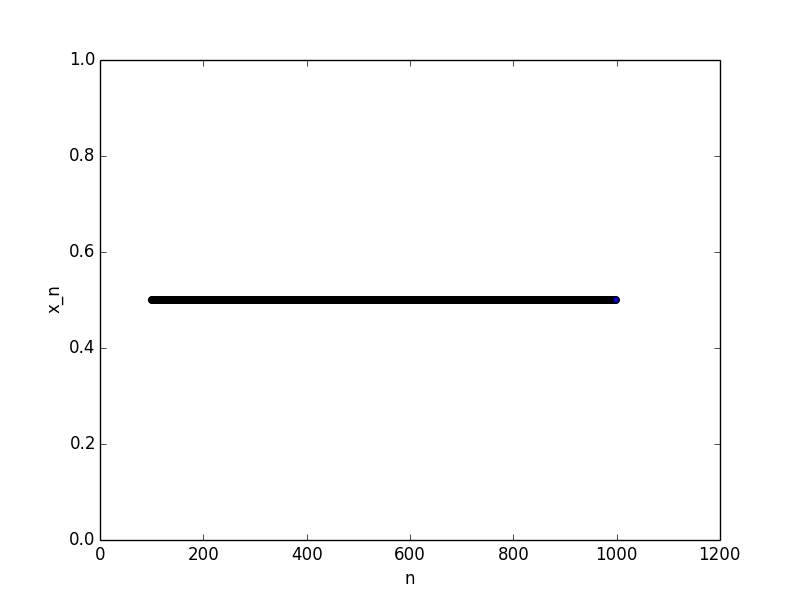
\includegraphics[scale = 0.4]{figs/R2_x0_02_fig1.png}
	\caption{The evolution of $x_{n}$ with $R = 2, x_{0} = 0.2$}
	\label{1}
\end{figure}

\subsubsection*{$R = 3.3, x_{0} = 0.2$}
With the coefficient $R = 2$ and the initial condition $x_{0} = 0.2$, we observe the 2-periodic cycle. In the fig.\ref{4} displaying the relationship between $x_{n+2}$ and $x_{n}$ we see two points sit on fixed points, which makes sense since the system is 2-periodic cycle, its state in the next 2 steps should be the same as the current state.


\begin{figure}
	\centering
	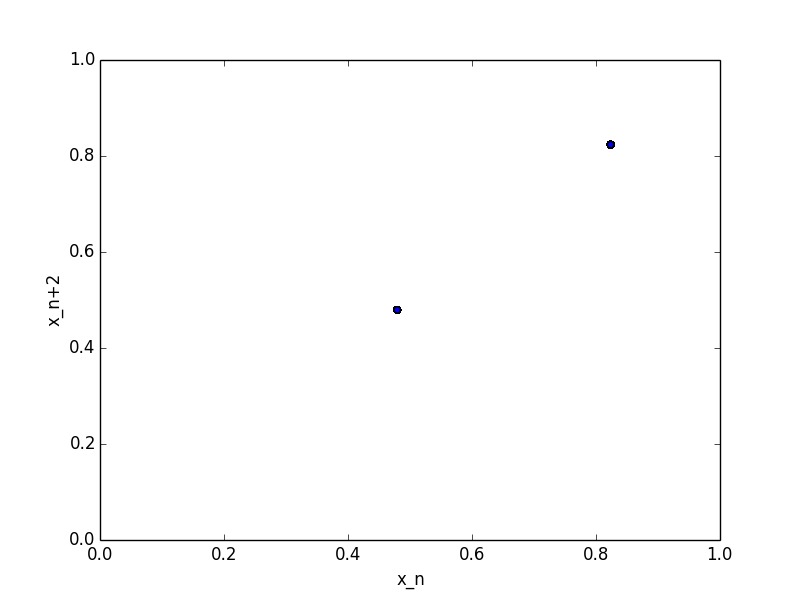
\includegraphics[scale = 0.4]{figs/R33_x0_02_fig3.png}
	\caption{$x_{n+2}$ versus $x_{n}$}
	\label{4}
\end{figure}

\subsubsection*{$R = 4.0, x_{0} = 0.2 \text{ and } x_{0} = 0.200001$ }
In order to see the chaotic behavior, we plot two trajectories with $R = 4.0$ for two different initial conditions, namely $x_{0} = 0.2$ and $x_{0} = 0.200001$. Only a difference of $0.000001$, two trajectories display very distinct behavior after $n = 15$.

\begin{figure}
	\centering
	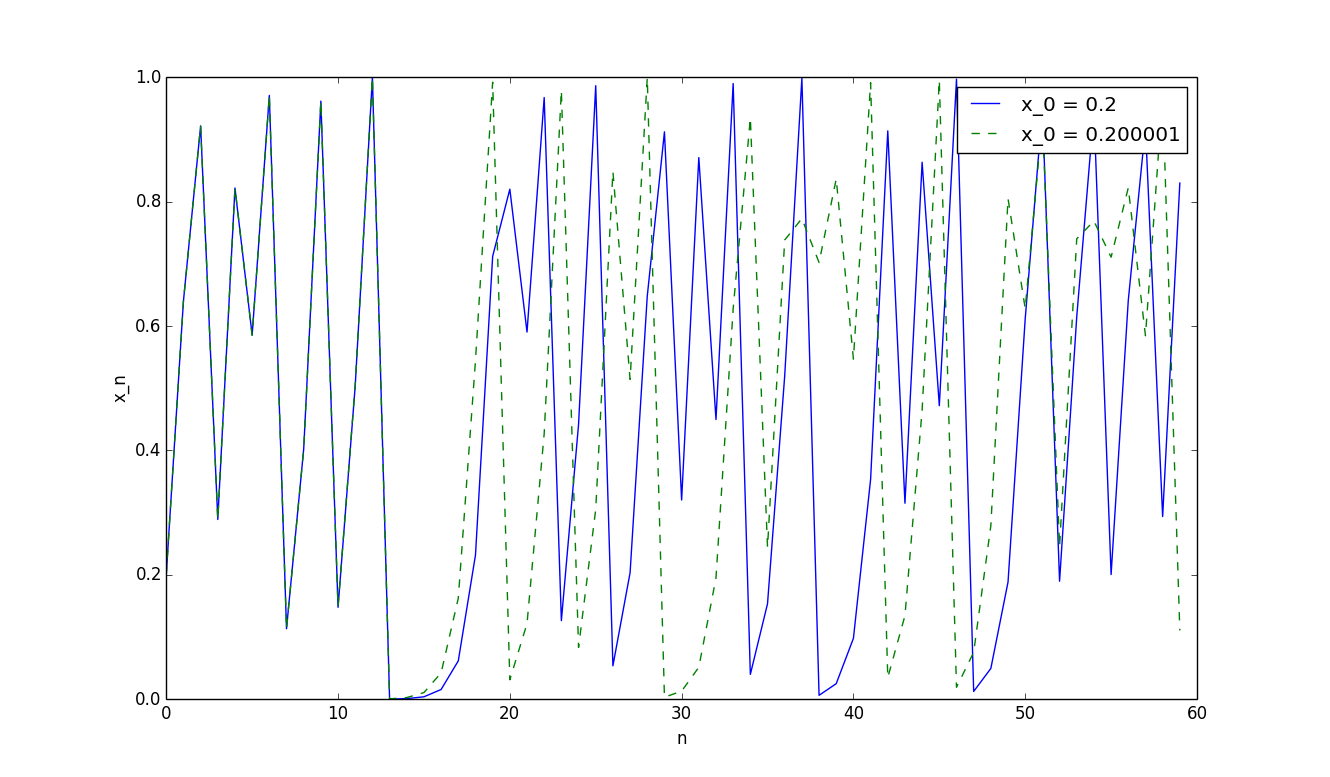
\includegraphics[scale = 0.4]{figs/two_trajectories_R4.png}
	\caption{Two trajectories for two different initial conditions.}
	\label{4}
\end{figure}

\subsubsection*{$R > 4.0$}
When $R > 4.0$, the value of $x_{n}$ diverges rapidly. In fig.\ref{divergence}, the output of logistic map with $R = 5$ and $x_{0} = 0.2$ is displayed on the standard output. Analytically, we can easily see that with these conditions, $x_{n}$ converges to a fixed point $0.8$. However, due to the precision of floating point in Python, after $x_{2}$, $x_{n}$ gradually deviates from 0.8, and it diverges rapidly after a certain point. This indicates that  when $R > 4.0$, fixed points are unstable, meaning that even a tiny deviation from them results in rapid divergence.

\subsubsection*{$R = 2.5$}
Any initial condition value $0 < x_{0} < 1$ eventually converges to 0.6. This set of initial conditions is called the basin of an attractor, which in this case $x_{n} = 0.6$.

\begin{figure}
	\centering
	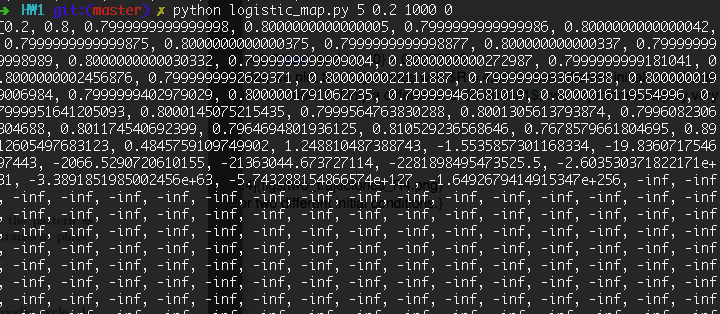
\includegraphics[scale = 0.4]{figs/screen_shot.png}
	\caption{Divergence of $x_{n}$ when $R = 5$ and $x_{0} = 0.2$.}
	\label{divergence}
\end{figure}

\end{document}












